\documentclass[t]{beamer}
\usepackage{mathtools}
\usepackage{tikz}
\usepackage{pgfplots}
\usepackage{ulem}
\usetikzlibrary{arrows,backgrounds,shapes,matrix,positioning,fit}
\newcommand{\argmax}{\operatornamewithlimits{argmax}}
\newcommand{\argmin}{\operatornamewithlimits{argmin}}
\newcommand{\wt}{\operatornamewithlimits{wt}}
\renewcommand\Re{\operatorname{Re}}
\renewcommand\Im{\operatorname{Im}}

\mode<presentation>
{
  \usetheme{Singapore}
  %\useoutertheme{infolines} % Showing only current section in navigation
  \setbeamertemplate{headline}{}  % Empty headline
  \setbeamertemplate{footline}[frame number]  % Getting rid of footer items except slide number
  \setbeamercovered{invisible}
  \beamertemplatenavigationsymbolsempty % Getting rid of navigation bullets at the bottom
}
\usepackage[english]{babel}
\usepackage[latin1]{inputenc}
\usepackage{times}
\usepackage[T1]{fontenc}

\title[EE 703 DMT]{Optimal Receiver for the AWGN Channel}
\author[Saravanan V]
{
  Saravanan Vijayakumaran\\
  \href{mailto:sarva@ee.iitb.ac.in}{sarva@ee.iitb.ac.in}
}
\institute[IIT Bombay]
{
  Department of Electrical Engineering\\
  Indian Institute of Technology Bombay
}
\date{September 23, 2013}

\AtBeginSection[]%
{%
\begin{frame}[plain]%
  \topskip0pt
  \vspace*{\fill}
    \begin{center}%
      \usebeamerfont{section title}\insertsection%
    \end{center}%
  \vspace*{\fill}
\end{frame}%
}

\begin{document}

\begin{frame}
  \titlepage
\end{frame}

%% Frame %%
\begin{frame}{Additive White Gaussian Noise Channel}
  \footnotesize
  \begin{figure}
    \centering
      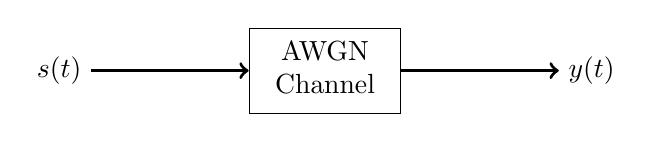
\begin{tikzpicture}[scale=1.0,transform shape]
        \node[rectangle, draw, minimum size = 5mm] (AWGN) {
                                                           \begin{tabular}{c}
                                                            AWGN \\
                                                            Channel
                                                           \end{tabular}
                                                          };
        \node[left = 2cm of AWGN] (st) {$s(t)$};
        \node[right = 2cm of AWGN] (rt) {$y(t)$};
        \draw[->,very thick] (st) -- (AWGN);
        \draw[->,very thick] (AWGN) -- (rt);
      \end{tikzpicture}
  \end{figure}
  \pause
  \begin{equation*}
    y(t) = s(t) + n(t)
  \end{equation*}
  \pause
  \begin{description}
    \item[$s(t)$] Transmitted Signal
    \pause
    \item[$y(t)$] Received Signal
    \pause
    \item[$n(t)$] White Gaussian Noise
  \end{description}
  \pause
  \begin{eqnarray*}
    S_n(f) = \frac{N_0}{2} = \sigma^2 
  \end{eqnarray*}
  \pause
  \begin{eqnarray*}
    R_n(\tau) = \sigma^2 \delta(\tau)
  \end{eqnarray*}
  \normalsize
\end{frame}

%% Frame %%
\begin{frame}{$M$-ary Signaling in AWGN Channel}
  \footnotesize
  \begin{itemize}
    \item One of $M$ continuous-time signals $s_1(t), \ldots, s_M(t)$ is sent
    \pause
    \item The received signal is the transmitted signal corrupted by AWGN
    \pause
    \item $M$ hypotheses with prior probabilities $\pi_i$, $i=1,\ldots,M$
      \begin{equation*}
        \begin{array}{ccc}
            H_1 & : & y(t) = s_1(t) + n(t) \\
            H_2 & : & y(t) = s_2(t) + n(t) \\
            \vdots &   &  \vdots          \\
            H_M & : & y(t) = s_M(t) + n(t) \\
        \end{array}
      \end{equation*}
    \pause
    \item Random variables are easier to handle than random processes
    \pause
    \item We derive an equivalent $M$-ary hypothesis testing problem involving only random vectors
  \end{itemize}
  \normalsize
\end{frame}

%% Frame %%
\begin{frame}{Restriction to Signal Space is Optimal}
  \footnotesize
  \begin{theorem}
    For the $M$-ary hypothesis testing given by
      \begin{equation*}
        \begin{array}{ccc}
            H_1 & : & y(t) = s_1(t) + n(t) \\
            \vdots &   &  \vdots          \\
            H_M & : & y(t) = s_M(t) + n(t) 
        \end{array}
      \end{equation*}
    there is no loss in detection performance by using the optimal
    decision rule for the following $M$-ary hypothesis testing problem
      \begin{equation*}
        \begin{array}{ccc}
            H_1 & : & \mathbf{Y} = \mathbf{s}_1 + \mathbf{N} \\
            \vdots &   &  \vdots          \\
            H_M & : & \mathbf{Y} = \mathbf{s}_M + \mathbf{N}
        \end{array}
      \end{equation*}
      where $\mathbf{Y}$, $\mathbf{s}_i$ and $\mathbf{N}$ are the projections of $y(t)$, $s_i(t)$ and $n(t)$ respectively onto the signal space spanned by $\{s_i(t)\}$.
  \end{theorem}
  \normalsize
\end{frame}

%% Frame %%
\begin{frame}{Projection of Signals onto Signal Space}
  \footnotesize
  \begin{itemize}
    \item Consider an orthonormal basis $\{\psi_i(t) | i=1,\ldots,K\}$ for the space spanned by $\{s_i(t)|i=1,\ldots,M\}$
    \item \pause Projection of $s_i(t)$ onto the signal space is
      \begin{equation*}
        \mathbf{s}_i = \begin{bmatrix} \langle s_i, \psi_1 \rangle & \cdots & \langle s_i, \psi_K \rangle \end{bmatrix}^T
      \end{equation*}
    \pause
    \begin{figure}
      \centering
        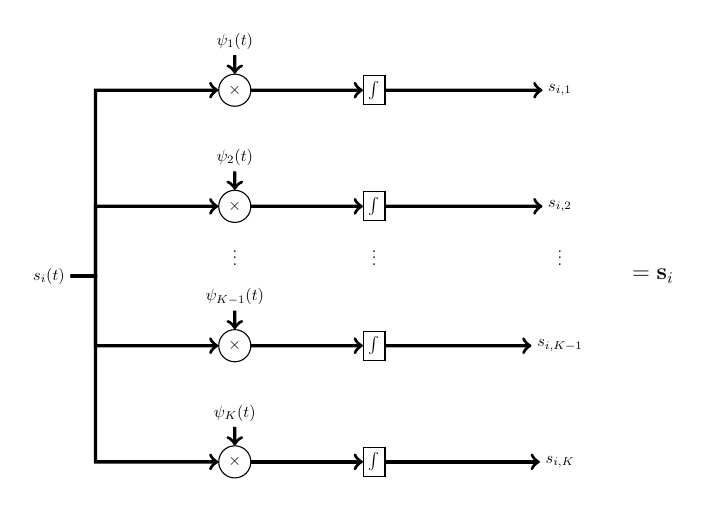
\begin{tikzpicture}[scale=0.59,transform shape]
          \tikzstyle{circblock}=[circle, draw]
          \tikzstyle{rectblock}=[rectangle, draw]
          \node at (-1,4) (st) {$s_i(t)$};
          \node at (12,4) (vecsi) {\Large $=\mathbf{s}_i$};
          \pause
          \node at (10,0) (sn) {$s_{i,K}$};
          \node at (10,2.5) (snm1) {$s_{i,K-1}$};
          \node at (10,4.5) (vdots1) {$\vdots$};
          \node at (10,5.5) (s2) {$s_{i,2}$};
          \node at (10,8) (s1) {$s_{i,1}$};
          \node[circblock] at (3,8) (prod1) {$\times$};
          \node[circblock] at (3,5.5) (prod2) {$\times$};
          \node at (3,4.5) (vdots2) {$\vdots$};
          \node[circblock] at (3,2.5) (prodnm1) {$\times$};
          \node[circblock] at (3,0) (prodn) {$\times$};
          \draw[->,very thick] (st) --++(1,0) |- (prod1);
          \draw[->,very thick] (st) --++(1,0) |- (prod2);
          \draw[->,very thick] (st) --++(1,0) |- (prodnm1);
          \draw[->,very thick] (st) --++(1,0) |- (prodn);
          \node[above=0.4 of prod1] (psi1) {$\psi_1(t)$};
          \node[above=0.4 of prod2] (psi2) {$\psi_2(t)$};
          \node[above=0.4 of prodnm1] (psinm1) {$\psi_{K-1}(t)$};
          \node[above=0.4 of prodn] (psin) {$\psi_K(t)$};
          \draw[->,very thick] (psi1) -- (prod1);
          \draw[->,very thick] (psi2) -- (prod2);
          \draw[->,very thick] (psinm1) -- (prodnm1);
          \draw[->,very thick] (psin) -- (prodn);
          \node[rectblock] at (6,0) (intn) {$\int$};
          \node[rectblock] at (6,2.5) (intnm1) {$\int$};
          \node at (6,4.5) (vdots3) {$\vdots$};
          \node[rectblock] at (6,5.5) (int2) {$\int$};
          \node[rectblock] at (6,8) (int1) {$\int$};
          \draw[->,very thick] (int1) -- (s1);
          \draw[->,very thick] (int2) -- (s2);
          \draw[->,very thick] (intnm1) -- (snm1);
          \draw[->,very thick] (intn) -- (sn);
          \draw[->,very thick] (prod1) -- (int1);
          \draw[->,very thick] (prod2) -- (int2);
          \draw[->,very thick] (prodnm1) -- (intnm1);
          \draw[->,very thick] (prodn) -- (intn);
        \end{tikzpicture}
    \end{figure}
  \end{itemize}
  \normalsize
\end{frame}

%% Frame %%
\begin{frame}{Projection of Observed Signal onto Signal Space}
  \footnotesize
  \begin{itemize}
    \item \pause Projection of $y(t)$ onto the signal space is
      \begin{equation*}
        \mathbf{Y} = \begin{bmatrix} \langle y, \psi_1 \rangle & \cdots & \langle y, \psi_K \rangle \end{bmatrix}^T 
      \end{equation*}
      \begin{figure}
        \centering
          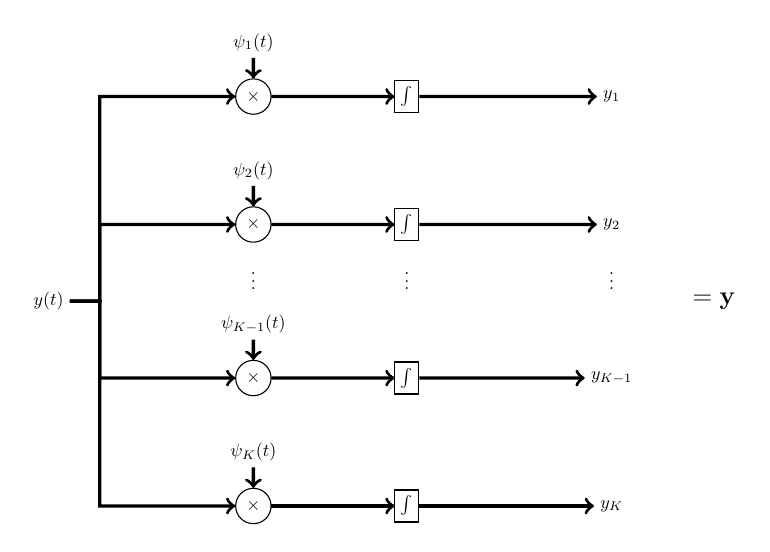
\begin{tikzpicture}[scale=0.65,transform shape]
            \tikzstyle{circblock}=[circle, draw]
            \tikzstyle{rectblock}=[rectangle, draw]
            \node at (-1,4) (yt) {$y(t)$};
            \node at (12,4) (vecsi) {\Large $=\mathbf{y}$};
            \pause
            \node at (10,0) (yn) {$y_{K}$};
            \node at (10,2.5) (ynm1) {$y_{K-1}$};
            \node at (10,4.5) (vdots1) {$\vdots$};
            \node at (10,5.5) (y2) {$y_{2}$};
            \node at (10,8) (y1) {$y_{1}$};
            \node[circblock] at (3,8) (prod1) {$\times$};
            \node[circblock] at (3,5.5) (prod2) {$\times$};
            \node at (3,4.5) (vdots2) {$\vdots$};
            \node[circblock] at (3,2.5) (prodnm1) {$\times$};
            \node[circblock] at (3,0) (prodn) {$\times$};
            \draw[->,very thick] (yt) --++(1,0) |- (prod1);
            \draw[->,very thick] (yt) --++(1,0) |- (prod2);
            \draw[->,very thick] (yt) --++(1,0) |- (prodnm1);
            \draw[->,very thick] (yt) --++(1,0) |- (prodn);
            \node[above=0.4 of prod1] (psi1) {$\psi_1(t)$};
            \node[above=0.4 of prod2] (psi2) {$\psi_2(t)$};
            \node[above=0.4 of prodnm1] (psinm1) {$\psi_{K-1}(t)$};
            \node[above=0.4 of prodn] (psin) {$\psi_K(t)$};
            \draw[->,very thick] (psi1) -- (prod1);
            \draw[->,very thick] (psi2) -- (prod2);
            \draw[->,very thick] (psinm1) -- (prodnm1);
            \draw[->,very thick] (psin) -- (prodn);
            \node[rectblock] at (6,0) (intn) {$\int$};
            \node[rectblock] at (6,2.5) (intnm1) {$\int$};
            \node at (6,4.5) (vdots3) {$\vdots$};
            \node[rectblock] at (6,5.5) (int2) {$\int$};
            \node[rectblock] at (6,8) (int1) {$\int$};
            \draw[->,very thick] (int1) -- (y1);
            \draw[->,very thick] (int2) -- (y2);
            \draw[->,very thick] (intnm1) -- (ynm1);
            \draw[->,very thick] (intn) -- (yn);
            \draw[->,very thick] (prod1) -- (int1);
            \draw[->,very thick] (prod2) -- (int2);
            \draw[->,very thick] (prodnm1) -- (intnm1);
            \draw[->,very thick] (prodn) -- (intn);
          \end{tikzpicture}
      \end{figure}
  \end{itemize}
  \normalsize
\end{frame}

%% Frame %%
\begin{frame}{Projection of Noise onto Signal Space}
  \footnotesize
  \begin{itemize}
    \item \pause Projection of $n(t)$ onto the signal space is
      \begin{equation*}
        \mathbf{N} = \begin{bmatrix} \langle n, \psi_1 \rangle & \cdots & \langle n, \psi_K \rangle \end{bmatrix}^T
      \end{equation*}
      \begin{figure}
        \centering
          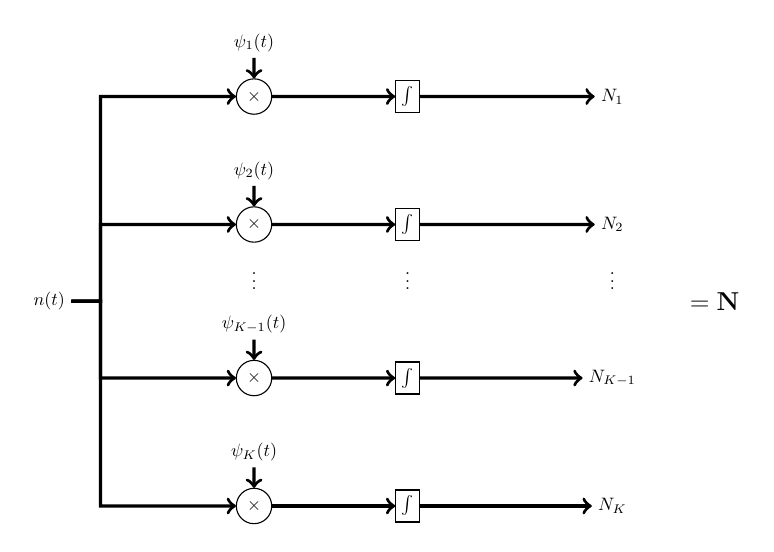
\begin{tikzpicture}[scale=0.65,transform shape]
            \tikzstyle{circblock}=[circle, draw]
            \tikzstyle{rectblock}=[rectangle, draw]
            \node at (-1,4) (nt) {$n(t)$};
            \node at (12,4) (vecsi) {\Large $=\mathbf{N}$};
            \pause
            \node at (10,0) (yn) {$N_{K}$};
            \node at (10,2.5) (ynm1) {$N_{K-1}$};
            \node at (10,4.5) (vdots1) {$\vdots$};
            \node at (10,5.5) (y2) {$N_{2}$};
            \node at (10,8) (y1) {$N_{1}$};
            \node[circblock] at (3,8) (prod1) {$\times$};
            \node[circblock] at (3,5.5) (prod2) {$\times$};
            \node at (3,4.5) (vdots2) {$\vdots$};
            \node[circblock] at (3,2.5) (prodnm1) {$\times$};
            \node[circblock] at (3,0) (prodn) {$\times$};
            \draw[->,very thick] (nt) --++(1,0) |- (prod1);
            \draw[->,very thick] (nt) --++(1,0) |- (prod2);
            \draw[->,very thick] (nt) --++(1,0) |- (prodnm1);
            \draw[->,very thick] (nt) --++(1,0) |- (prodn);
            \node[above=0.4 of prod1] (psi1) {$\psi_1(t)$};
            \node[above=0.4 of prod2] (psi2) {$\psi_2(t)$};
            \node[above=0.4 of prodnm1] (psinm1) {$\psi_{K-1}(t)$};
            \node[above=0.4 of prodn] (psin) {$\psi_K(t)$};
            \draw[->,very thick] (psi1) -- (prod1);
            \draw[->,very thick] (psi2) -- (prod2);
            \draw[->,very thick] (psinm1) -- (prodnm1);
            \draw[->,very thick] (psin) -- (prodn);
            \node[rectblock] at (6,0) (intn) {$\int$};
            \node[rectblock] at (6,2.5) (intnm1) {$\int$};
            \node at (6,4.5) (vdots3) {$\vdots$};
            \node[rectblock] at (6,5.5) (int2) {$\int$};
            \node[rectblock] at (6,8) (int1) {$\int$};
            \draw[->,very thick] (int1) -- (y1);
            \draw[->,very thick] (int2) -- (y2);
            \draw[->,very thick] (intnm1) -- (ynm1);
            \draw[->,very thick] (intn) -- (yn);
            \draw[->,very thick] (prod1) -- (int1);
            \draw[->,very thick] (prod2) -- (int2);
            \draw[->,very thick] (prodnm1) -- (intnm1);
            \draw[->,very thick] (prodn) -- (intn);
          \end{tikzpicture}
      \end{figure}
  \end{itemize}
  \normalsize
\end{frame}



%% Frame %%
\begin{frame}{Proof of Theorem}
  \footnotesize
  \begin{itemize}
    \item $\mathbf{Y} = \begin{bmatrix} \langle y, \psi_1 \rangle & \cdots & \langle y, \psi_K \rangle \end{bmatrix}^T$
    \item \pause Component of $y(t)$ orthogonal to the signal space is
      \begin{equation*}
        y^{\perp}(t) = y(t) - \sum_{i=1}^K \langle y, \psi_i \rangle \psi_i(t)
      \end{equation*}
    \item \pause $y(t)$ is equivalent to $(\mathbf{Y}, y^{\perp}(t))$
    \item \pause We claim that $y^\perp(t)$ is an irrelevant statistic \pause
      \begin{eqnarray*}
        y^{\perp}(t) & = & y(t) - \sum_{i=1}^K \langle y, \psi_i \rangle \psi_i(t)\\
                     \pause
                     & = & s_i(t) + n(t) - \sum_{j=1}^K\langle s_i+n, \psi_j \rangle \psi_j(t) \\
                     \pause
                     & = & n(t) - \sum_{j=1}^K\langle n,\psi_j\rangle \psi_j(t)  \pause = n^{\perp}(t)
      \end{eqnarray*}
      where $n^\perp(t)$ is the component of $n(t)$ orthogonal to the signal space.
    \item \pause $n^{\perp}(t)$ is independent of which $s_i(t)$ was transmitted which makes $y^\perp(t)$ an irrelevant statistic.
  \end{itemize}
  \normalsize
\end{frame}

%% Frame %%
\begin{frame}{$M$-ary Signaling in AWGN Channel}
  \footnotesize
  \begin{itemize}
    \item $M$ hypotheses with prior probabilities $\pi_i$, $i=1,\ldots,M$
      \begin{equation*}
        \begin{array}{ccc}
            H_1 & : & \mathbf{Y} = \mathbf{s}_1 + \mathbf{N} \\
            \vdots &   &  \vdots          \\
            H_M & : & \mathbf{Y} = \mathbf{s}_M + \mathbf{N}
        \end{array}
      \end{equation*}
      \pause
      \begin{eqnarray*}
        \mathbf{Y} & = & \begin{bmatrix} \langle y, \psi_1 \rangle & \cdots & \langle y, \psi_K \rangle \end{bmatrix}^T \\
        \pause
        \mathbf{s}_i & = & \begin{bmatrix} \langle s_i, \psi_1 \rangle & \cdots & \langle s_i, \psi_K \rangle \end{bmatrix}^T \\
        \pause
        \mathbf{N} & = & \begin{bmatrix} \langle n, \psi_1 \rangle & \cdots & \langle n, \psi_K \rangle \end{bmatrix}^T
      \end{eqnarray*}
    \item \pause $\mathbf{N} \sim N(\mathbf{m}, \mathbf{C})$ \pause where $\mathbf{m} = \pause \mathbf{0}$ and $\mathbf{C} = \pause \sigma^2 \mathbf{I}$
      \begin{equation*}
        \pause \text{cov}\left( \langle n, \psi_1 \rangle, \langle n, \psi_2 \rangle \right) = \pause \sigma^2 \langle \psi_1, \psi_2 \rangle.
      \end{equation*}
  \end{itemize}
  \normalsize
\end{frame}

%% Frame %%
\begin{frame}{Optimal Receiver for the AWGN Channel}
  \footnotesize
  \begin{theorem}[MPE Decision Rule]
    The MPE decision rule for $M$-ary signaling in AWGN channel is given by
      \begin{eqnarray*}
        \delta_{MPE}(\mathbf{y}) & = & \pause \argmin_{1 \leq i \leq M} \lVert \mathbf{y} - \mathbf{s}_i \rVert^2 - 2\sigma^2\log \pi_i \\
        \pause
                                 & = & \argmax_{1 \leq i \leq M} \langle \mathbf{y}, \mathbf{s}_i \rangle - \frac{\lVert \mathbf{s}_i \rVert^2}{2} +\sigma^2\log \pi_i 
        \pause
      \end{eqnarray*}
  \end{theorem}
  \begin{block}{Proof}
      \begin{eqnarray*}
        \delta_{MPE}(\mathbf{y}) & = & \pause \argmax_{1 \leq i \leq M} \pi_i p_i(\mathbf{y}) \\
                                 & = & \pause \argmax_{1 \leq i \leq M} \pi_i \exp\left( -\frac{\lVert \mathbf{y}-\mathbf{s}_i\rVert^2}{2\sigma^2}\right)
      \end{eqnarray*}
  \end{block}
  \normalsize
\end{frame}

%% Frame %%
\begin{frame}{MPE Decision Rule}
  \footnotesize
  \pause
  \begin{figure}
    \centering
      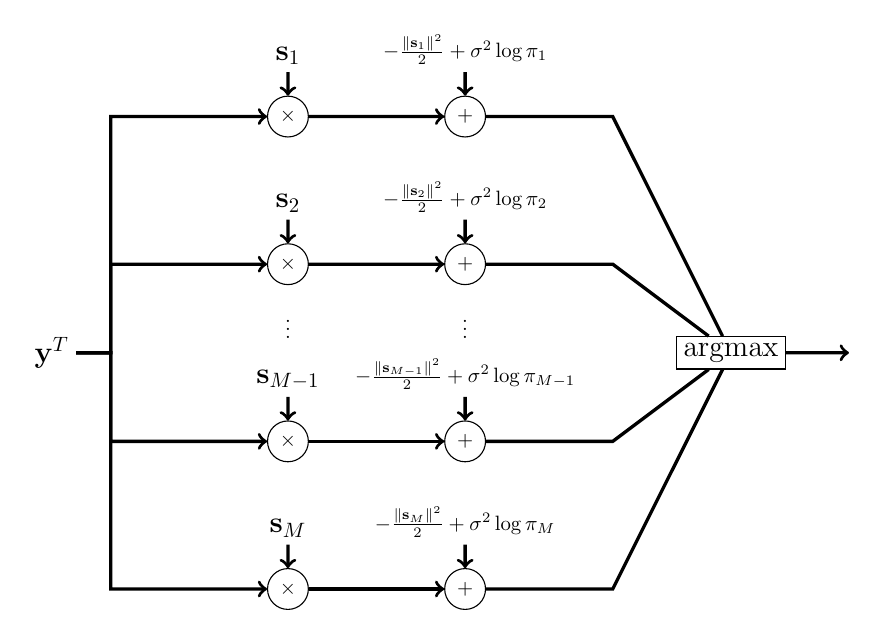
\begin{tikzpicture}[scale=0.75,transform shape]
        \tikzstyle{circblock}=[circle, draw]
        \tikzstyle{rectblock}=[rectangle, draw]
        \node at (-1,4) (yvec) {\Large $\mathbf{y}^T$};
        \node[circblock] at (3,8) (prod1) {$\times$};
        \node[circblock] at (3,5.5) (prod2) {$\times$};
        \node at (3,4.5) (vdots2) {$\vdots$};
        \node[circblock] at (3,2.5) (prodMm1) {$\times$};
        \node[circblock] at (3,0) (prodM) {$\times$};
        \draw[->,very thick] (yvec) --++(1,0) |- (prod1);
        \draw[->,very thick] (yvec) --++(1,0) |- (prod2);
        \draw[->,very thick] (yvec) --++(1,0) |- (prodMm1);
        \draw[->,very thick] (yvec) --++(1,0) |- (prodM);
        \pause
        \node[above=0.4 of prod1] (s1) {\Large $\mathbf{s}_1$};
        \node[above=0.4 of prod2] (s2) {\Large $\mathbf{s}_2$};
        \node[above=0.4 of prodMm1] (sMm1) {\Large $\mathbf{s}_{M-1}$};
        \node[above=0.4 of prodM] (sM) {\Large $\mathbf{s}_M$};
        \draw[->,very thick] (s1) -- (prod1);
        \draw[->,very thick] (s2) -- (prod2);
        \draw[->,very thick] (sMm1) -- (prodMm1);
        \draw[->,very thick] (sM) -- (prodM);
        \pause
        \node[circblock] at (6,0) (plusM) {$+$};
        \node[circblock] at (6,2.5) (plusMm1) {$+$};
        \node at (6,4.5) (vdots3) {$\vdots$};
        \node[circblock] at (6,5.5) (plus2) {$+$};
        \node[circblock] at (6,8) (plus1) {$+$};
        \draw[->,very thick] (prod1) -- (plus1);
        \draw[->,very thick] (prod2) -- (plus2);
        \draw[->,very thick] (prodMm1) -- (plusMm1);
        \draw[->,very thick] (prodM) -- (plusM);
        \pause
        \node[above=0.4 of plus1] (c1) { $-\frac{\lVert \mathbf{s}_1 \rVert^2}{2} + \sigma^2\log \pi_1$};
        \node[above=0.4 of plus2] (c2) {$-\frac{\lVert \mathbf{s}_2 \rVert^2}{2} + \sigma^2\log \pi_2$};
        \node[above=0.4 of plusMm1] (cMm1) {$-\frac{\lVert \mathbf{s}_{M-1} \rVert^2}{2} + \sigma^2\log \pi_{M-1}$};
        \node[above=0.4 of plusM] (cM) {$-\frac{\lVert \mathbf{s}_M \rVert^2}{2} + \sigma^2\log \pi_M$};
        \draw[->,very thick] (c1) -- (plus1);
        \draw[->,very thick] (c2) -- (plus2);
        \draw[->,very thick] (cMm1) -- (plusMm1);
        \draw[->,very thick] (cM) -- (plusM);
        \pause
        \node[rectblock] at (10.5,4) (max) {\Large $\argmax$};
        \draw[-,very thick] (plus1) -- (8.5,8) -- (max);
        \draw[-,very thick] (plus2) -- (8.5,5.5) -- (max);
        \draw[-,very thick] (plusMm1) -- (8.5,2.5) -- (max);
        \draw[-,very thick] (plusM) -- (8.5,0) -- (max);
        \draw[->, very thick] (max) -- (12.5,4);
      \end{tikzpicture}
  \end{figure}
  \normalsize
\end{frame}

%% Frame %%
\begin{frame}{Continuous-Time Version of MPE Rule}
  \footnotesize
  \begin{itemize}
    \item Discrete-time version
      \begin{eqnarray*}
        \delta_{MPE}(\mathbf{y}) & = & \argmax_{1 \leq i \leq M} \langle \mathbf{y}, \mathbf{s}_i \rangle - \frac{\lVert \mathbf{s}_i \rVert^2}{2} +\sigma^2\log \pi_i
      \end{eqnarray*}
    \pause
    \item Continuous-time version
      \begin{eqnarray*}
        \delta_{MPE}(y) & = & \argmax_{1 \leq i \leq M} \langle y, s_i \rangle - \frac{\lVert s_i \rVert^2}{2} +\sigma^2\log \pi_i
      \end{eqnarray*}
  \end{itemize}
  \normalsize
\end{frame}

%% Frame %%
\begin{frame}{MPE Decision Rule Example}
  \footnotesize
  \begin{figure}[h]
    \centering
      \begin{tikzpicture}[scale=0.45,transform shape]
        \begin{axis}[
                     title=$s_1(t)$,
                     xmax=3.5,
                     xmin=0,
                     ymax=2.5,
                     ymin=-1.5,
                     axis lines = middle,
                     ytick={2,0},
                     xtick = {0,1,2,3,3.5},
                     xticklabels = {$0$,1,2,3,$t$},
                     yticklabels = {2,0},
                    ]
          \addplot[color=blue,very thick] coordinates {(0,2) (3,2) (3,0) };
        \end{axis}
      \end{tikzpicture}
    \centering
      \begin{tikzpicture}[scale=0.45,transform shape]
        \begin{axis}[
                     title=$s_2(t)$,
                     xmax=3.5,
                     xmin=0,
                     ymax=2.5,
                     ymin=-1.5,
                     axis lines = middle,
                     ytick={2,0},
                     xtick = {0,1,3.5},
                     xticklabels = {$0$,1,$t$},
                     yticklabels = {2,0},
                    ]
          \addplot[color=blue,very thick] coordinates {(0,2) (1,2) (1,0)};
        \end{axis}
      \end{tikzpicture}
    \centering
      \begin{tikzpicture}[scale=0.45,transform shape]
        \begin{axis}[
                     title=$s_3(t)$,
                     xmax=3.5,
                     xmin=0,
                     ymax=1.5,
                     ymin=-2.5,
                     axis lines = middle,
                     ytick={0, -2},
                     xtick = {0,1,2,3,3.5},
                     xticklabels = {$0$,1,2,3,$t$},
                     xticklabel shift = -20pt,
                     yticklabels = {0,-2},
                    ]
          \addplot[color=blue,very thick] coordinates {(1,0) (1,-2) (3,-2) (3,0)};
        \end{axis}
      \end{tikzpicture}
    \centering
      \begin{tikzpicture}[scale=0.45,transform shape]
        \begin{axis}[
                     title=$s_4(t)$,
                     xmax=3.5,
                     xmin=0,
                     ymax=2.5,
                     ymin=-1.5,
                     axis lines = middle,
                     ytick={2,0},
                     xtick = {0,1,2,3,3.5},
                     xticklabels = {$0$,1,2,3,$t$},
                     yticklabels = {2,0},
                    ]
          \addplot[color=blue,very thick] coordinates {(0,2) (2,2) (2,0)};
        \end{axis}
      \end{tikzpicture}
    \centering
      \begin{tikzpicture}[scale=0.45,transform shape]
        \begin{axis}[
                     title=$y(t)$,
                     xmax=3.5,
                     xmin=0,
                     ymax=2.5,
                     ymin=-1.5,
                     axis lines = middle,
                     ytick={2,1,0},
                     xtick = {0,1,2,3,3.5},
                     xticklabels = {$0$,1,2,3,$t$},
                     yticklabels = {2,1,0},
                    ]
          \addplot[color=red,very thick] coordinates {(0,2) (1,2) (1,0) (2,0) (2,2) (3,2) (3,0)};
        \end{axis}
      \end{tikzpicture}
  \end{figure}
  \begin{equation*}
    \text{Let } \pi_1 = \pi_2 = \frac{1}{3}, \pi_3 = \pi_4 = \frac{1}{6}, \sigma^2 = 1, \text{ and } \log 2 = 0.69.
  \end{equation*}
  \normalsize
\end{frame}

%% Frame %%
\begin{frame}{ML Receiver for the AWGN Channel}
  \footnotesize
  \begin{theorem}[ML Decision Rule]
    The ML decision rule for $M$-ary signaling in AWGN channel is given by
      \begin{eqnarray*}
        \delta_{ML}(\mathbf{y}) & = & \pause \argmin_{1 \leq i \leq M} \lVert \mathbf{y} - \mathbf{s}_i \rVert^2 \\
        \pause
                                 & = & \argmax_{1 \leq i \leq M} \langle \mathbf{y}, \mathbf{s}_i \rangle - \frac{\lVert \mathbf{s}_i \rVert^2}{2}
      \end{eqnarray*}
  \end{theorem}
  \pause
  \begin{block}{Proof}
      \begin{eqnarray*}
        \delta_{ML}(\mathbf{y}) & = & \pause \argmax_{1 \leq i \leq M} p_i(\mathbf{y}) \\
                                 & = & \pause \argmax_{1 \leq i \leq M} \exp\left( -\frac{\lVert \mathbf{y}-\mathbf{s}_i\rVert^2}{2\sigma^2}\right)
      \end{eqnarray*}
  \end{block}
  \normalsize
\end{frame}

%% Frame %%
\begin{frame}{ML Decision Rule}
  \footnotesize
  \pause
  \begin{figure}
    \centering
      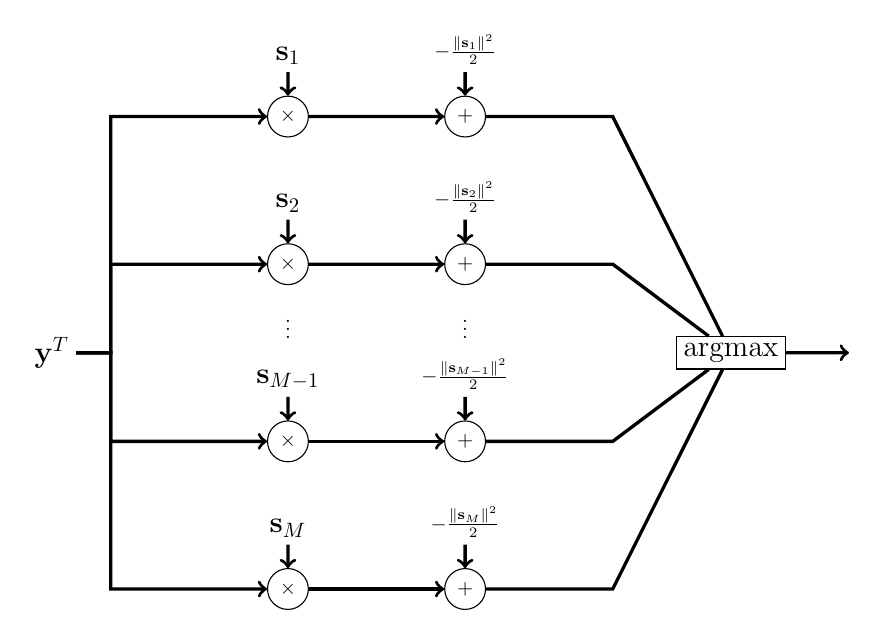
\begin{tikzpicture}[scale=0.75,transform shape]
        \tikzstyle{circblock}=[circle, draw]
        \tikzstyle{rectblock}=[rectangle, draw]
        \node at (-1,4) (yvec) {\Large $\mathbf{y}^T$};
        \node[circblock] at (3,8) (prod1) {$\times$};
        \node[circblock] at (3,5.5) (prod2) {$\times$};
        \node at (3,4.5) (vdots2) {$\vdots$};
        \node[circblock] at (3,2.5) (prodMm1) {$\times$};
        \node[circblock] at (3,0) (prodM) {$\times$};
        \draw[->,very thick] (yvec) --++(1,0) |- (prod1);
        \draw[->,very thick] (yvec) --++(1,0) |- (prod2);
        \draw[->,very thick] (yvec) --++(1,0) |- (prodMm1);
        \draw[->,very thick] (yvec) --++(1,0) |- (prodM);
        \pause
        \node[above=0.4 of prod1] (s1) {\Large $\mathbf{s}_1$};
        \node[above=0.4 of prod2] (s2) {\Large $\mathbf{s}_2$};
        \node[above=0.4 of prodMm1] (sMm1) {\Large $\mathbf{s}_{M-1}$};
        \node[above=0.4 of prodM] (sM) {\Large $\mathbf{s}_M$};
        \draw[->,very thick] (s1) -- (prod1);
        \draw[->,very thick] (s2) -- (prod2);
        \draw[->,very thick] (sMm1) -- (prodMm1);
        \draw[->,very thick] (sM) -- (prodM);
        \pause
        \node[circblock] at (6,0) (plusM) {$+$};
        \node[circblock] at (6,2.5) (plusMm1) {$+$};
        \node at (6,4.5) (vdots3) {$\vdots$};
        \node[circblock] at (6,5.5) (plus2) {$+$};
        \node[circblock] at (6,8) (plus1) {$+$};
        \draw[->,very thick] (prod1) -- (plus1);
        \draw[->,very thick] (prod2) -- (plus2);
        \draw[->,very thick] (prodMm1) -- (plusMm1);
        \draw[->,very thick] (prodM) -- (plusM);
        \pause
        \node[above=0.4 of plus1] (c1) { $-\frac{\lVert \mathbf{s}_1 \rVert^2}{2}$};
        \node[above=0.4 of plus2] (c2) {$-\frac{\lVert \mathbf{s}_2 \rVert^2}{2}$};
        \node[above=0.4 of plusMm1] (cMm1) {$-\frac{\lVert \mathbf{s}_{M-1} \rVert^2}{2}$};
        \node[above=0.4 of plusM] (cM) {$-\frac{\lVert \mathbf{s}_M \rVert^2}{2}$};
        \draw[->,very thick] (c1) -- (plus1);
        \draw[->,very thick] (c2) -- (plus2);
        \draw[->,very thick] (cMm1) -- (plusMm1);
        \draw[->,very thick] (cM) -- (plusM);
        \pause
        \node[rectblock] at (10.5,4) (max) {\Large $\argmax$};
        \draw[-,very thick] (plus1) -- (8.5,8) -- (max);
        \draw[-,very thick] (plus2) -- (8.5,5.5) -- (max);
        \draw[-,very thick] (plusMm1) -- (8.5,2.5) -- (max);
        \draw[-,very thick] (plusM) -- (8.5,0) -- (max);
        \draw[->, very thick] (max) -- (12.5,4);
      \end{tikzpicture}
  \end{figure}
  \normalsize
\end{frame}

%% Frame %%
\begin{frame}{ML Decision Rule}
  \footnotesize
  \pause
  \begin{figure}
    \centering
      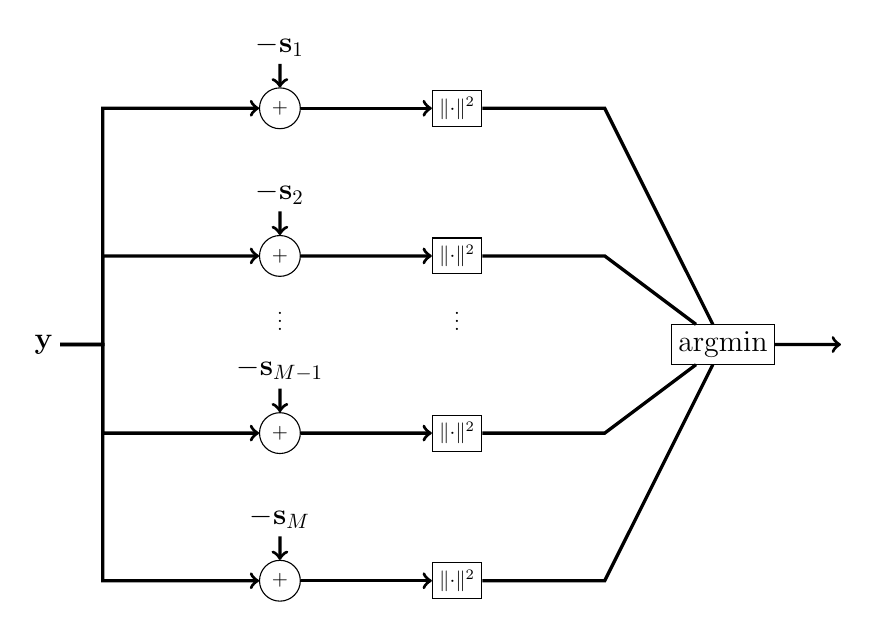
\begin{tikzpicture}[scale=0.75,transform shape]
        \tikzstyle{circblock}=[circle, draw]
        \tikzstyle{rectblock}=[rectangle, draw]
        \node at (-1,4) (yvec) {\Large $\mathbf{y}$};
        \node[circblock] at (3,8) (sub1) {$+$};
        \node[circblock] at (3,5.5) (sub2) {$+$};
        \node at (3,4.5) (vdots2) {$\vdots$};
        \node[circblock] at (3,2.5) (subMm1) {$+$};
        \node[circblock] at (3,0) (subM) {$+$};
        \draw[->,very thick] (yvec) --++(1,0) |- (sub1);
        \draw[->,very thick] (yvec) --++(1,0) |- (sub2);
        \draw[->,very thick] (yvec) --++(1,0) |- (subMm1);
        \draw[->,very thick] (yvec) --++(1,0) |- (subM);
        \node[above=0.4 of sub1] (s1) {\Large $-\mathbf{s}_1$};
        \node[above=0.4 of sub2] (s2) {\Large $-\mathbf{s}_2$};
        \node[above=0.4 of subMm1] (sMm1) {\Large $-\mathbf{s}_{M-1}$};
        \node[above=0.4 of subM] (sM) {\Large $-\mathbf{s}_M$};
        \draw[->,very thick] (s1) -- (sub1);
        \draw[->,very thick] (s2) -- (sub2);
        \draw[->,very thick] (sMm1) -- (subMm1);
        \draw[->,very thick] (sM) -- (subM);
        \pause
        \node[rectblock] at (6,0) (normM) {$\lVert \cdot \rVert^2$};
        \node[rectblock] at (6,2.5) (normMm1) {$\lVert \cdot \rVert^2$};
        \node at (6,4.5) (vdots3) {$\vdots$};
        \node[rectblock] at (6,5.5) (norm2) {$\lVert \cdot \rVert^2$};
        \node[rectblock] at (6,8) (norm1) {$\lVert \cdot \rVert^2$};
        \draw[->,very thick] (sub1) -- (norm1);
        \draw[->,very thick] (sub2) -- (norm2);
        \draw[->,very thick] (subMm1) -- (normMm1);
        \draw[->,very thick] (subM) -- (normM);
        \pause
        \node[rectblock] at (10.5,4) (min) {\Large $\argmin$};
        \draw[-,very thick] (norm1) -- (8.5,8) -- (min);
        \draw[-,very thick] (norm2) -- (8.5,5.5) -- (min);
        \draw[-,very thick] (normMm1) -- (8.5,2.5) -- (min);
        \draw[-,very thick] (normM) -- (8.5,0) -- (min);
        \draw[->, very thick] (min) -- (12.5,4);
      \end{tikzpicture}
  \end{figure}
  \normalsize
\end{frame}

%% Frame %%
\begin{frame}{Continuous-Time Version of ML Rule}
  \footnotesize
  \begin{itemize}
    \item Discrete-time version
      \begin{eqnarray*}
        \delta_{ML}(\mathbf{y}) & = & \argmax_{1 \leq i \leq M} \langle \mathbf{y}, \mathbf{s}_i \rangle - \frac{\lVert \mathbf{s}_i \rVert^2}{2}
      \end{eqnarray*}
    \pause
    \item Continuous-time version
      \begin{eqnarray*}
        \delta_{ML}(y) & = & \argmax_{1 \leq i \leq M} \langle y, s_i \rangle - \frac{\lVert s_i \rVert^2}{2}
      \end{eqnarray*}
  \end{itemize}
  \normalsize
\end{frame}

%% Frame %%
\begin{frame}{ML Decision Rule Example}
  \footnotesize
  \begin{figure}[h]
    \centering
      \begin{tikzpicture}[scale=0.45,transform shape]
        \begin{axis}[
                     title=$s_1(t)$,
                     xmax=3.5,
                     xmin=0,
                     ymax=2.5,
                     ymin=-1.5,
                     axis lines = middle,
                     ytick={2,0},
                     xtick = {0,1,2,3,3.5},
                     xticklabels = {$0$,1,2,3,$t$},
                     yticklabels = {2,0},
                    ]
          \addplot[color=blue,very thick] coordinates {(0,2) (3,2) (3,0) };
        \end{axis}
      \end{tikzpicture}
    \centering
      \begin{tikzpicture}[scale=0.45,transform shape]
        \begin{axis}[
                     title=$s_2(t)$,
                     xmax=3.5,
                     xmin=0,
                     ymax=2.5,
                     ymin=-1.5,
                     axis lines = middle,
                     ytick={2,0},
                     xtick = {0,1,3.5},
                     xticklabels = {$0$,1,$t$},
                     yticklabels = {2,0},
                    ]
          \addplot[color=blue,very thick] coordinates {(0,2) (1,2) (1,0)};
        \end{axis}
      \end{tikzpicture}
    \centering
      \begin{tikzpicture}[scale=0.45,transform shape]
        \begin{axis}[
                     title=$s_3(t)$,
                     xmax=3.5,
                     xmin=0,
                     ymax=1.5,
                     ymin=-2.5,
                     axis lines = middle,
                     ytick={0, -2},
                     xtick = {0,1,2,3,3.5},
                     xticklabels = {$0$,1,2,3,$t$},
                     xticklabel shift = -20pt,
                     yticklabels = {0,-2},
                    ]
          \addplot[color=blue,very thick] coordinates {(1,0) (1,-2) (3,-2) (3,0)};
        \end{axis}
      \end{tikzpicture}
    \centering
      \begin{tikzpicture}[scale=0.45,transform shape]
        \begin{axis}[
                     title=$s_4(t)$,
                     xmax=3.5,
                     xmin=0,
                     ymax=2.5,
                     ymin=-1.5,
                     axis lines = middle,
                     ytick={2,0},
                     xtick = {0,1,2,3,3.5},
                     xticklabels = {$0$,1,2,3,$t$},
                     yticklabels = {2,0},
                    ]
          \addplot[color=blue,very thick] coordinates {(0,2) (2,2) (2,0)};
        \end{axis}
      \end{tikzpicture}
    \centering
      \begin{tikzpicture}[scale=0.45,transform shape]
        \begin{axis}[
                     title=$y(t)$,
                     xmax=3.5,
                     xmin=0,
                     ymax=2.5,
                     ymin=-1.5,
                     axis lines = middle,
                     ytick={2,0},
                     xtick = {0,1,2,3,3.5},
                     xticklabels = {$0$,1,2,3,$t$},
                     yticklabels = {2,0},
                    ]
          \addplot[color=red,very thick] coordinates {(0,2) (1,2) (1,0) (2,0) (2,2) (3,2) (3,0)};
        \end{axis}
      \end{tikzpicture}
  \end{figure}
  \normalsize
\end{frame}

%% Frame %%
\begin{frame}{ML Decision Rule for Antipodal Signaling}
  \footnotesize
  \begin{figure}[h]
    \centering
      \begin{tikzpicture}[scale=0.45,transform shape]
        \begin{axis}[
                     title=$s_1(t)$,
                     xmax=3.5,
                     xmin=0,
                     ymax=2.5,
                     ymin=-2.5,
                     axis lines = middle,
                     ytick={2,0},
                     xtick = {0,1,2,3,3.5},
                     xticklabels = {$0$,,,$T$,$t$},
                     yticklabels = {$A$,0},
                    ]
          \addplot[color=blue,very thick] coordinates {(0,0) (3,2) (3,0) };
        \end{axis}
      \end{tikzpicture}
    \centering
      \begin{tikzpicture}[scale=0.45,transform shape]
        \begin{axis}[
                     title=$s_2(t)$,
                     xmax=3.5,
                     xmin=0,
                     ymax=2.5,
                     ymin=-2.5,
                     axis lines = middle,
                     ytick={-2,0},
                     xtick = {0,1,2,3,3.5},
                     xticklabels = {$0$,,,$T$,$t$},
                     yticklabels = {-$A$,0},
                     xticklabel shift = -20pt
                    ]
          \addplot[color=blue,very thick] coordinates {(0,0) (3,-2) (3,0)};
        \end{axis}
      \end{tikzpicture}
      \pause
      \begin{equation*}
        \delta_{ML}(y)  =  \pause \argmax_{1 \leq i \leq 2} \langle y, s_i \rangle - \frac{\lVert s_i \rVert^2}{2}  =  \pause \argmax_{1 \leq i \leq 2} \langle y, s_i \rangle
      \pause
      \end{equation*}
      $\delta_{ML}(y)  = 1 \iff \pause \langle y, s_1 \rangle \geq \pause \langle y, s_2 \rangle \pause \iff \langle y,s_1\rangle \geq 0$ \pause
      \begin{equation*}
        \langle y, s_1 \rangle =  \int_{0}^{T} y(\tau) s_1(\tau) \ d\tau \pause = (y\star s_{MF}) (T)
      \end{equation*}
      where $s_{MF}(t) = s_1(T-t)$ is the matched filter.
  \end{figure}
  \normalsize
\end{frame}

%% Frame %%
\begin{frame}{}
\vfill
\begin{center}
Thanks for your attention
\end{center}
\vfill
\end{frame}

\end{document}
